\chapter{Boilerplate for Sorting}
\section{Insertion Sort}
\begin{lstlisting}
void InsertionSort(std::vector<int>& nums) {
  for (int j = 1; j < nums.size(); ++j) {
    int insert_val = nums[j];
    int i = j - 1;
    while (i >= 0 && nums[i] > insert_val) {
      nums[i + 1] = nums[i];
      --i;
    }
    nums[i + 1] = insert_val;
  }
}
\end{lstlisting}
\begin{figure}[H]
	\centering
	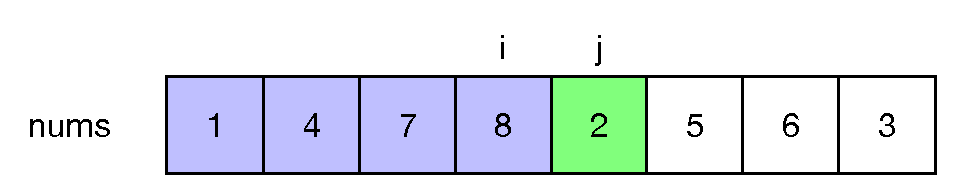
\includegraphics[width=0.5\linewidth]{images/insertion_sort}
	\caption{Insertion Sort}
	\label{fig:insertionsort}
\end{figure}

\section{Merge Sort}\label{merge_sort}
\begin{lstlisting}
void MergeSort(std::vector<int>& nums) {
  MergeSortRecursive(nums, 0, nums.size() - 1);
}

void MergeSortRecursive(std::vector<int>& nums, int start, int end) {
  if (start >= end) { return; }
  int mid = start + (end - start) / 2;
  MergeSortRecursive(nums, start, mid);
  MergeSortRecursive(nums, mid + 1, end);
  Merge(nums, start, mid, end);
}

void Merge(std::vector<int>& nums, int start, int mid, int end) {
  std::vector<int> tmp(end - start + 1);
  int i = start;
  int j = mid + 1;
  int k = 0;
  while (i <= mid && j <= end) {
    if (nums[i] < nums[j]) {
      tmp[k++] = nums[i++];
    } else {
      tmp[k++] = nums[j++];
    }
  }
  while (i <= mid) { tmp[k++] = nums[i++]; }
  while (j <= end) { tmp[k++] = nums[j++]; }
  for (int i = 0; i < tmp.size(); ++i) { nums[start + i] = tmp[i]; }
}
\end{lstlisting}

\begin{figure}[H]
	\centering
	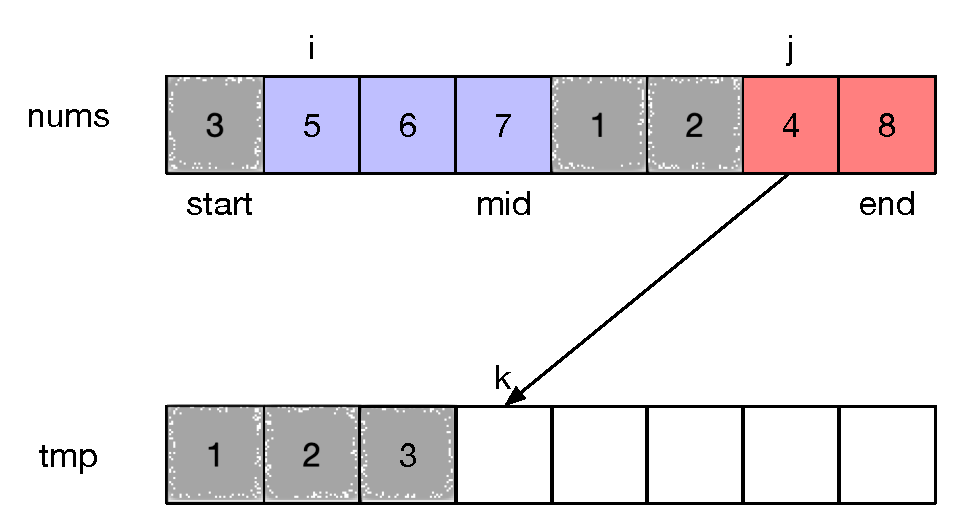
\includegraphics[width=0.5\linewidth]{images/merge_sort}
	\caption{Merge Sort - Merge}
	\label{fig:mergesort}
\end{figure}

\subsection*{Related}
\begin{itemize}
	\item \hyperref[lc0088]{LC 0088 - Merge Sorted Array}
	\item \hyperref[lc0021]{LC 0021 - Merge Two Sorted Lists}
	\item \hyperref[merge_sort]{Merge Sort}
\end{itemize}

\section{Quick Sort}\label{quick_sort}
\begin{lstlisting}
void QuickSort(std::vector<int>& nums) {
  QuickSortRecursive(nums, 0, nums.size() - 1);
}

void QuickSortRecursive(std::vector<int>& nums, int start, int end) {
  if (start >= end) { return; }
  int pivot_idx = Partition(nums, start, end);
  QuickSortRecursive(nums, start, pivot_idx - 1);
  QuickSortRecursive(nums, pivot_idx + 1, end);
}

int Partition(std::vector<int>& nums, int start, int end) {
  int pivot = nums[end];
  int i = start - 1;
  for (int j = start; j < end; ++j) {
    if (nums[j] <= pivot) {
      ++i;
      std::swap(nums[i], nums[j]);
    }
  }
  std::swap(nums[i + 1], nums[end]);
  return i + 1;
}
\end{lstlisting}

\subsection*{Related}
\begin{itemize}
	\item \hyperref[lc0086]{LC 0086 - Partition List}
	\item \hyperref[quick_sort]{Quick Sort}
\end{itemize}

\begin{figure}[H]
	\centering
	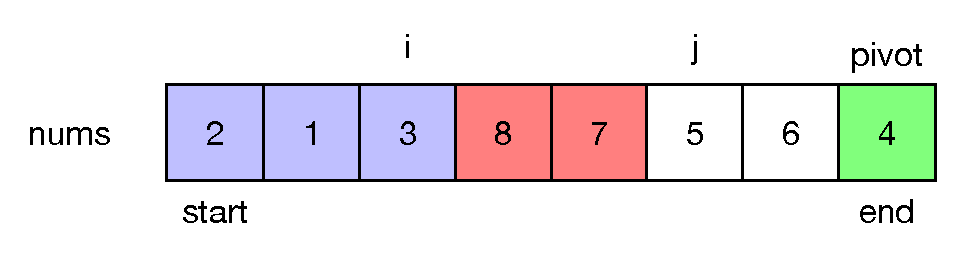
\includegraphics[width=0.5\linewidth]{images/quick_sort}
	\caption{Quick Sort - Partition}
	\label{fig:quicksort}
\end{figure}

\section{Heap Sort}\label{sec:heap_sort}
\begin{lstlisting}
void HeapSort(std::vector<int>& nums) {
  int n = nums.size();
  for (int i = n / 2 - 1; i >= 0; --i) { Heapify(nums, n, i); }
  for (int i = n - 1; i > 0; --i) {
    std::swap(nums[0], nums[i]);
    Heapify(nums, i, 0);
  }
}

void Heapify(std::vector<int>& nums, int n, int i) {
  int largest = i;
  int l = 2 * i + 1;
  int r = 2 * i + 2;
  if (l < n && nums[l] > nums[largest]) { largest = l; }
  if (r < n && nums[r] > nums[largest]) { largest = r; }
  if (largest != i) {
    std::swap(nums[i], nums[largest]);
    Heapify(nums, n, largest);
  }
}
\end{lstlisting}